\documentclass[12pt]{article}

% Packages
\usepackage[utf8]{inputenc}
\usepackage{amsmath}
\usepackage{amssymb}
\usepackage{graphicx}
\usepackage{hyperref}
\usepackage{geometry}
\usepackage{float}

% remove the indent at the beginning of a paragraph:
\setlength{\parindent}{0pt}

% Line spacing
\renewcommand{\baselinestretch}{1}

% distance between new paragraphs:
\setlength{\parskip}{0.5em}

% Title design:
\usepackage{titling}
\pretitle{\begin{center}\LARGE\bfseries}
\posttitle{\par\end{center}\vspace{-0.5em}}
\preauthor{\begin{center}\large}
\postauthor{\par\end{center}\vspace{-2em}}
\predate{\begin{center}\large}
\postdate{\par\end{center}\vspace{-1em}}


% Geometry settings
\geometry{
    a4paper,
    total={170mm,257mm},
    left=20mm,
    right=20mm,
    top=20mm,
    bottom=20mm,
}

% Set the figure counter to reset within subsections
\counterwithin{figure}{subsection}

% Document
\begin{document}

% Title Page
\title{Homework 2: Active Learning + GNNs}
\author{Naomi Derel 325324994, Gili Cohen 326280815, Renana Shachak 213920010}
\date{01.08.2024}
\maketitle

\section{Active Learning}

\subsection{Pipeline Structure}

The pipeline we used for active learning is as follows:
\begin{enumerate}
    \item Load the dataset and split it into train and test indices. Find the features and labels from the dataset.
    \item For a set number of iterations:
    \begin{itemize}
        \item Train a model on the labeled set.
        \item Use the model to predict the labels of the unlabeled set, and calculate an accuracy score.
        \item Select a number of samples from the unlabeled set according to a budget, using one of the selection methods as set. Update the labeled set with the new samples.
    \end{itemize}
    \item Output the accuracy scores for each iteration. Alternatively, output the final trained model.
\end{enumerate}

\subsection{Uncertainty-Based Selection}

The measure we picked for uncertainty-based selection is entropy. 

The entropy of a distribution is a measure of the uncertainty in that distribution, and so it is a classical measure for our case. 

We used it by calculating the entropy of the output of the model for each sample in the pool, and defining them as an estimate for the uncertainty of the model on that sample. We then selected the samples with the highest entropy to be labeled next, since they are the samples the model is most uncertain about.

\subsection{Custom Selection}

The measure we picked for custom selection is the density selection measure we saw in class.

the density selection is based upon the intuition that the model will benefit the most from samples that extend the vector space the model has seen so far. We used it by calculating the distance of each sample in the pool from the samples the model has seen so far, and then selecting the samples with the lowest density.

For defining the density measure, we tried two approaches (where $x_i$ are the samples the model has seen so far, and $x$ is the sample we are calculating the density for):

\begin{enumerate}
    \item The lowest sum of distances from the samples the model has seen: $ \sum_{i=1}^{n} distance(x_i, x) $.
    \item A density measure based on the sum of exponential distances from the samples the model has seen so far: $ \sum_{i=1}^{n} \exp(-distance(x_i, x)) $.
    This is based on a Gaussian kernel, and is a common measure for density.
\end{enumerate}
The first approach ended up achieving identical or better results, so we used it for the final implementation.

We then selected the samples with the highest density to be labeled next.

\subsection{Parameter Comparison}

We compared the results of multiple combinations of models, iterations, and budget per iteration as instructed. We defined pairs of iterations and budget per iteration to be under the limit of 600.

The following tables contain the final accuracy score for each combination. In bold, we present the best results by model, and underlined are the best results overall per selection method.

\subsubsection*{Random Selection}

\begin{table}[H]
    \centering
    \begin{tabular}{|c|c|c|c|}
        \hline
        & SVC & Random Forest & Logistic Regression \\
        \hline
        10 Iterations + 59 Budget & \textbf{0.686} & 0.677 & 0.675 \\
        15 Iterations + 39 Budget & 0.684 & 0.684 & \textbf{0.695} \\
        30 Iterations + 19 Budget & 0.682 & \underline{\textbf{0.699}} & 0.682 \\
        \hline
    \end{tabular}
    \caption{Results of Parameter Comparison for Random Selection}
\end{table}

\subsubsection*{Uncertainty-Based Selection}

\begin{table}[H]
    \centering
    \begin{tabular}{|c|c|c|c|}
        \hline
        & SVC & Random Forest & Logistic Regression \\
        \hline
        10 Iterations + 59 Budget & \underline{\textbf{0.699}} & \underline{\textbf{0.699}} & \underline{\textbf{0.699}} \\
        15 Iterations + 39 Budget & 0.688 & 0.688 & 0.688 \\
        30 Iterations + 19 Budget & 0.695 & 0.695 & 0.695 \\
        \hline
    \end{tabular}
    \caption{Results of Parameter Comparison for Uncertainty-Based Selection}
\end{table}


\subsubsection*{Custom Selection}

\begin{table}[H]
    \centering
    \begin{tabular}{|c|c|c|c|}
        \hline
        & SVC & Random Forest & Logistic Regression \\
        \hline
        10 Iterations + 59 Budget & 0.733 & 0.733 & 0.733 \\
        15 Iterations + 39 Budget & 0.729 & 0.729 & 0.729 \\
        30 Iterations + 19 Budget & \underline{\textbf{0.746}} & \underline{\textbf{0.746}} & \underline{\textbf{0.746}} \\
        \hline
    \end{tabular}
    \caption{Results of Parameter Comparison for Custom Selection}
\end{table}

\subsubsection*{Comparison by Selection}

We now compare the training process for the model which achieved the best results of each selection method. For the selections with tied results, we chose to show the Random Forest model for consistency.

\begin{figure}[H]
    \centering
    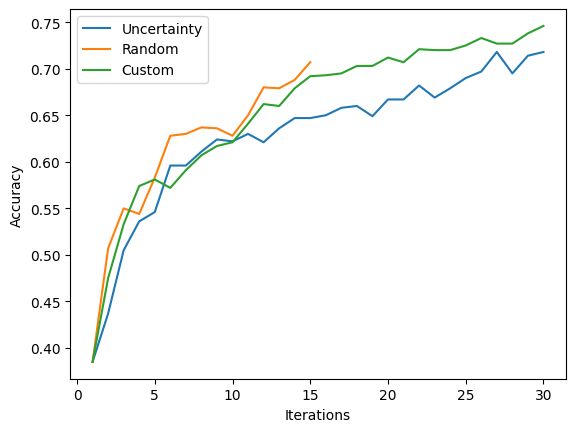
\includegraphics[width=0.8\textwidth]{criterion_comparison.png}
    \caption{Comparison of Training Process for Best Results by Selection Method}
\end{figure}

Overall, we can see the custom criterion with 30 iterations and 19 budget per iteration achieved the best results, with an accuracy score of 0.746 (regardless of the model used).

\subsubsection*{Analysis and Discussion}

The results show a few interesting points. Firstly, when using an advanced selection method (not random), the chosen model does not affect the results but the combination of iterations and budget per iteration does. This might mean that the models are equally good at learning from the data, but the selection method and iterations are key to the success of the active learning process.

Secondly, while the custom selection method achieved the best results with more iterations and a lower budget per iteration, the uncertainty-based selection method was directly opposite, achieving the best results with fewer iterations and a higher budget per iteration (but with a lower difference in accuracy scores). Consistently, the middle ground of the the tradeoff between iterations and budget per iteration was the worst for both selection methods.

Specifically for our custom selection method based on density, we can see that the model benefits from a lower budget per iteration, which seems to be better for an understanding of the data distribution. It benefits from more iterations, which allows the model more time to learn from the data. In contrast, the uncertainty-based selection method benefits from a higher budget per iteration, which allows the model to learn from more samples at once which might be more beneficial if the uncertainty signal is weak.

 The random selection model, however, has changes in performance based both on the model used and the combination of iterations and budget. The winner among iterations per models changes with random effects, but the random forest model with most iterations seemed to consistently perform best overall. This is surprising, since overall this method has sees the lowest number of samples, but this could be due to the randomness of the selection.

 Lastly, the plot of the training process for the best models per selection method shows that the uncertainty-based selection reaches better results faster (with more budget per iteration), but the custom selection method reaches better results with a more steady increase. The random method behaves more similarly to the custom method and sometimes even outperforms it during training, but eventually falls behind.

% % Table of Contents
% \tableofcontents
% \newpage

% % Bibliography
% \newpage
% \begin{thebibliography}{99}
%     \bibitem{ref1} Author, \emph{Title}, Publisher, Year.
%     \bibitem{ref2} Author, \emph{Title}, Publisher, Year.
%     % Add more references as needed
% \end{thebibliography}

\end{document}